%!TEX root = ../main/main.tex
\section{User Interface View} % (fold)
\label{sec:user_interface_view}
This section focuses on the user interface point of view using UX UML diagram to specify the possible interactions and the flow of events.\\
Layouts for the applications are described and outlined in \emph{section 3.1} of the \emph{RASD}.\\
% section user_interface_view (end)

\vfill
\begin{figure}[h!t]
\caption{User App Login UX}
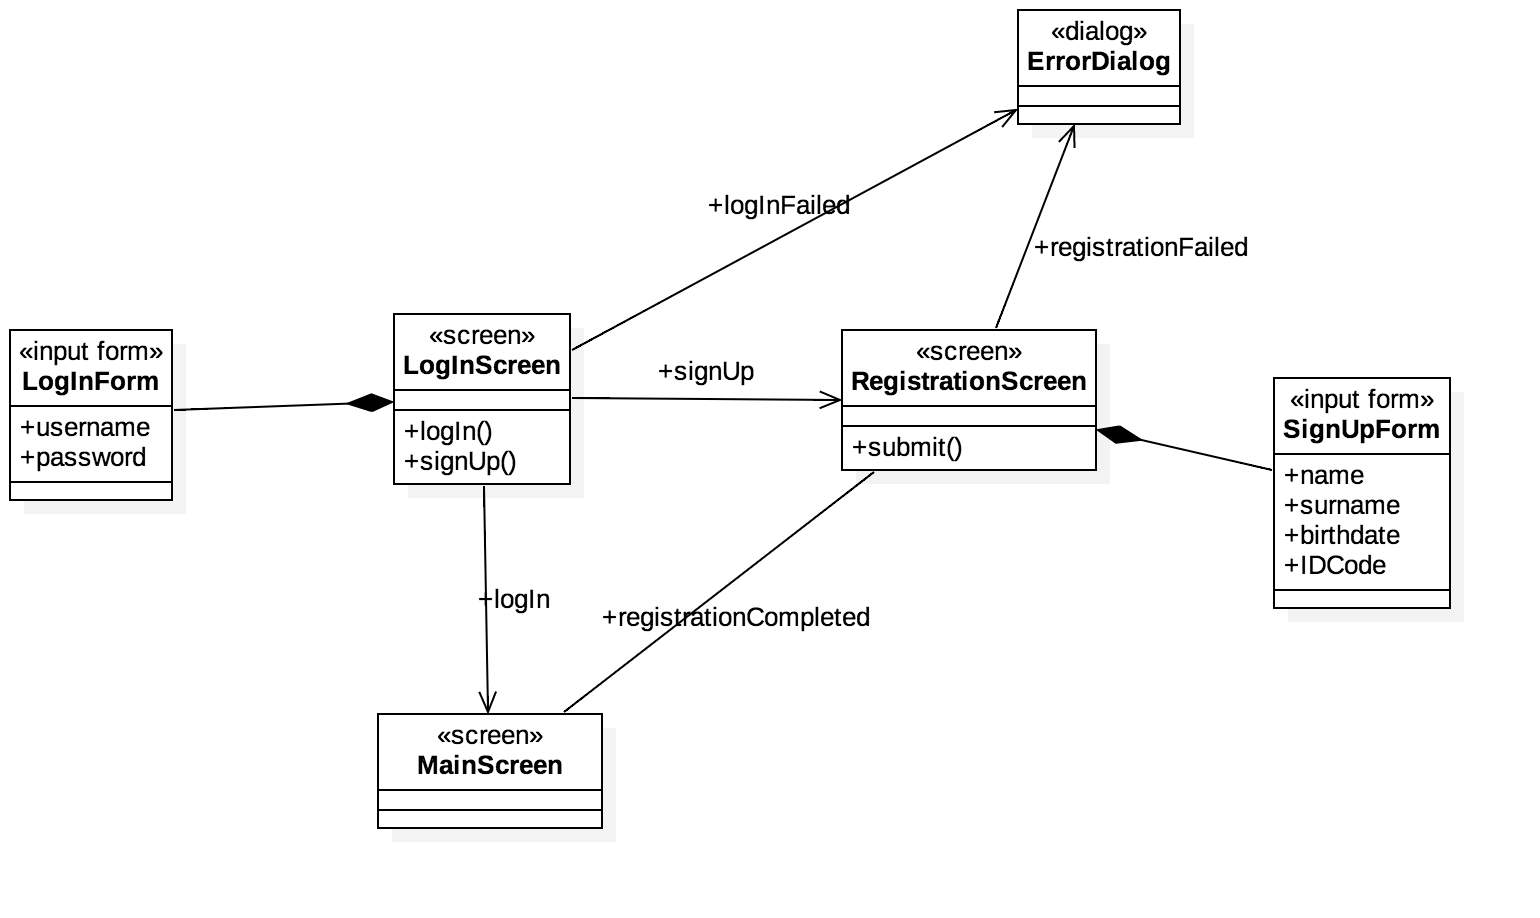
\includegraphics[width=\textwidth]{diagram/png/loginUXUser}
\centering
\end{figure}
\vfill
\clearpage

\newpage
\vfill
\begin{figure}[h!t]
\caption{User App MainScreen UX}
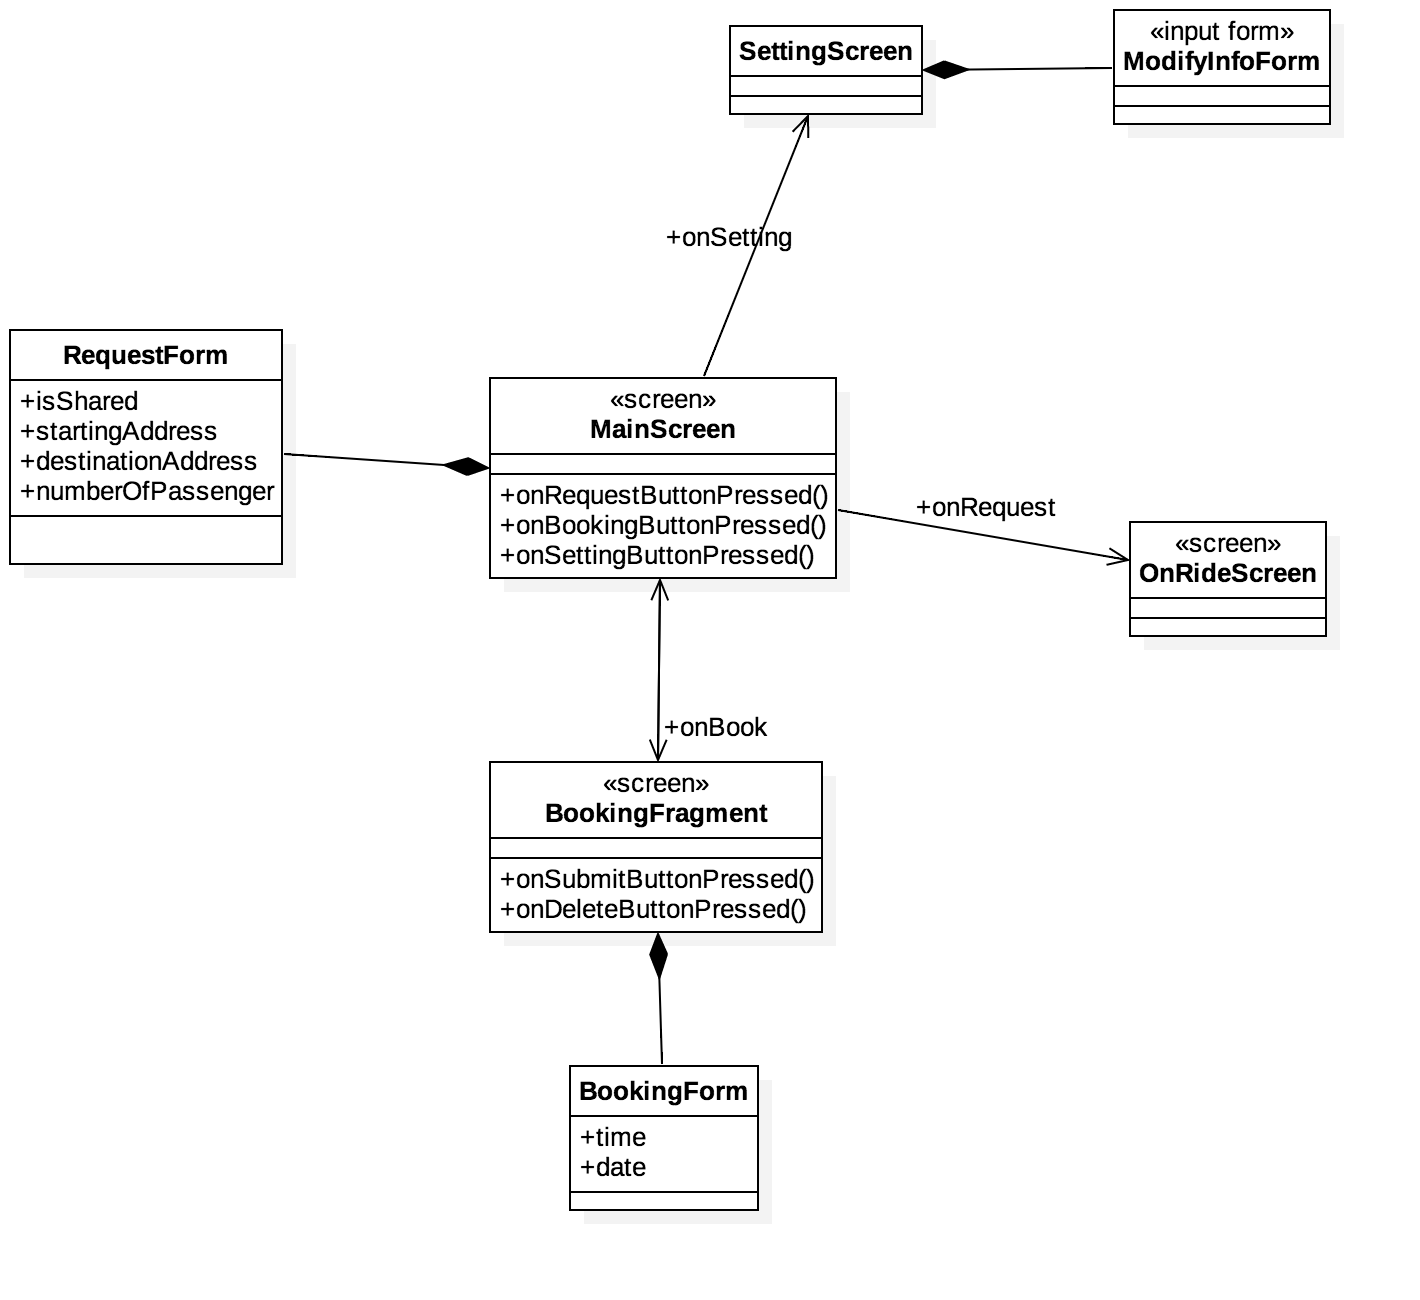
\includegraphics[width=\textwidth]{diagram/png/mainScreenUXUser}
\centering
\end{figure}
\vfill
\clearpage

\newpage
\vfill
\begin{figure}[h!t]
\caption{User App On Ride Screen UX}
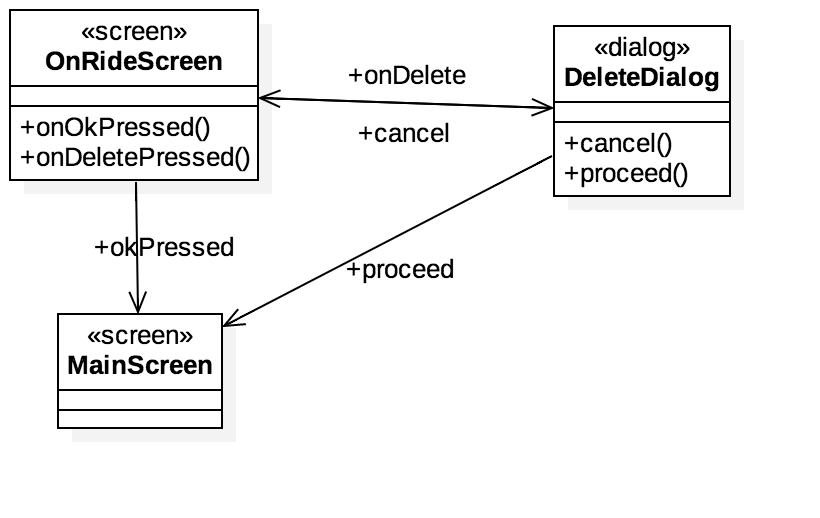
\includegraphics[width=\textwidth]{diagram/png/onRideScreenUX}
\centering
\end{figure}
\vfill
\clearpage

\newpage
\vfill
\begin{figure}[h!t]
\caption{Taxi Driver App Login UX}
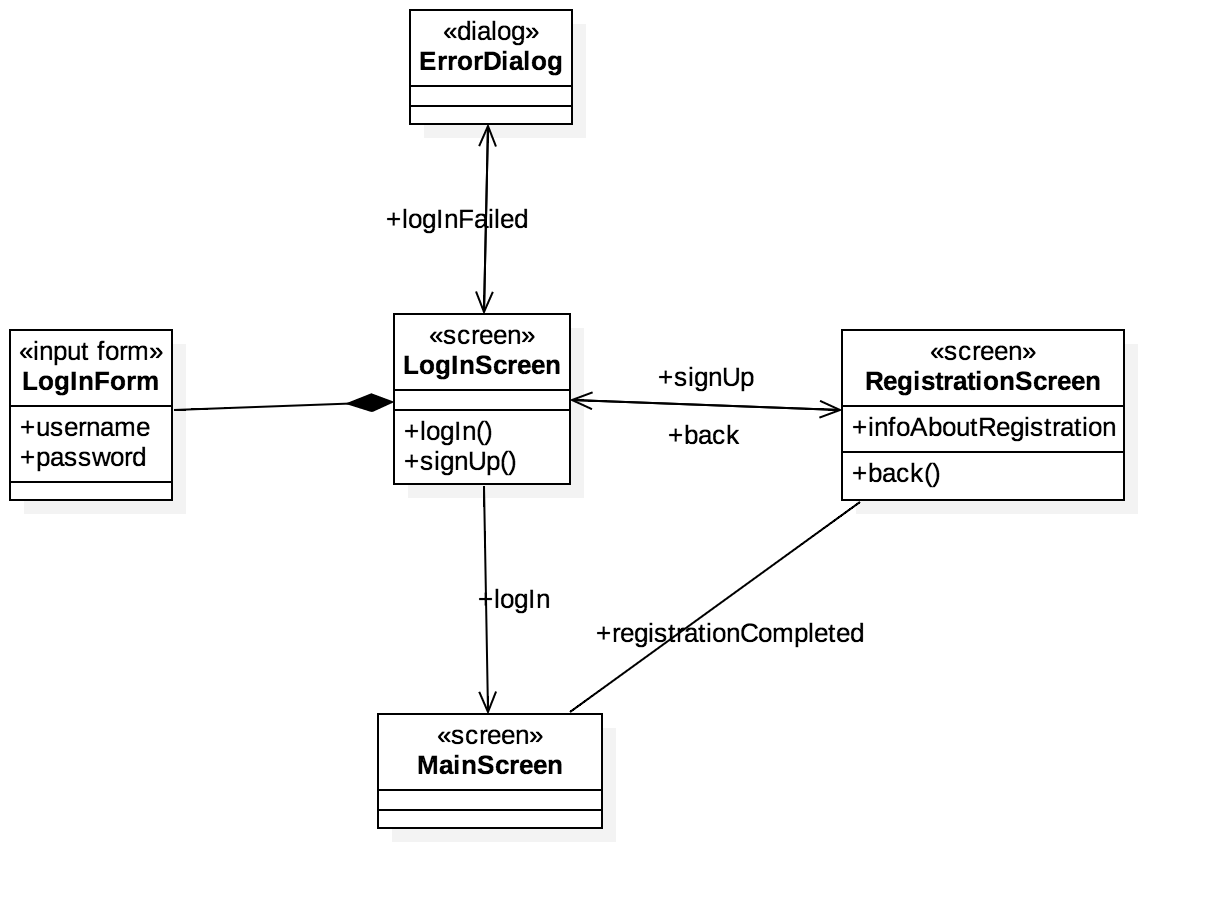
\includegraphics[width=\textwidth]{diagram/png/loginUXDriver}
\centering
\end{figure}
\vfill
\clearpage


\newpage
\vfill
\begin{figure}[h!t]
\caption{Taxi Driver App MainScreen UX}
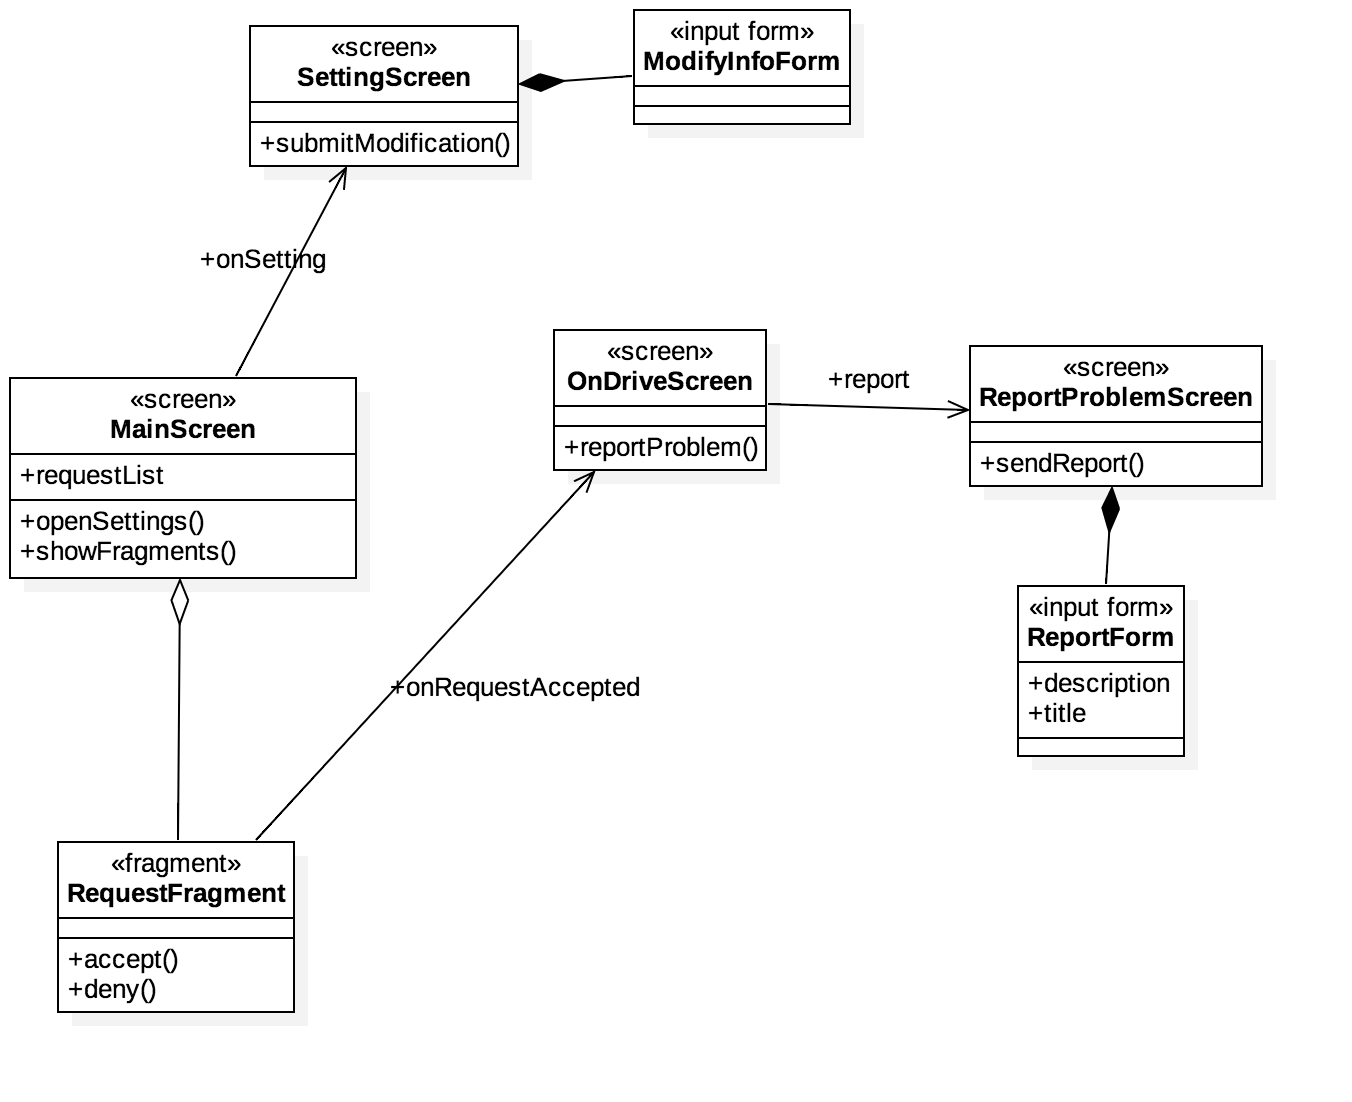
\includegraphics[width=\textwidth]{diagram/png/mainScreeUXDriver}
\centering
\end{figure}
\vfill
\clearpage